\section{Application Mobile Livreur}

\subsection{Rôle de la partie mobile}

L'application mobile constitue l'interface dédiée aux livreurs du projet GoMile. Elle leur permet de:
\begin{itemize}
    \item créer un compte et finaliser l'activation,
    \item consulter et accepter des missions,
    \item suivre une livraison avec vérification par code,
    \item gérer leur profil, leur disponibilité et leurs documents KYC.
\end{itemize}

Cette partie a été développée en React Native avec Expo et Expo Go pour accélérer les itérations et faciliter les démonstrations sur téléphone pendant le projet.

\subsection{Architecture générale et technologies}

L'application mobile repose sur les briques suivantes:
\begin{description}
    \item[React Navigation] gestion des écrans d'authentification et des onglets principaux.
    \item[Expo] accès aux fonctionnalités natives (média, géolocalisation, notifications) avec un cycle de développement rapide.
    \item[API backend GoMile] authentification, missions, profil, vérification et opérations métier.
    \item[Modules externes] \texttt{@react-native-community/datetimepicker} pour la date, composants média pour photo/document, services d'adressage pour fiabiliser les adresses.
\end{description}

\subsubsection{Pourquoi Zustand avant de décrire les étapes}

Le flux d'inscription traverse plusieurs écrans successifs. Les données doivent donc être partagées entre écrans, conservées pendant la navigation, et réutilisées au moment de l'appel API final. Pour cette raison, nous avons retenu \texttt{Zustand} (\texttt{useRegistrationStore}) plutôt qu'un simple objet JavaScript local à un écran. Ce choix apporte:
\begin{itemize}
    \item un état centralisé lisible,
    \item des mises à jour champ par champ,
    \item une meilleure robustesse si l'utilisateur revient à l'étape précédente.
\end{itemize}

La description détaillée des champs arrive ensuite, pour montrer concrètement ce qui est stocké à chaque étape.

\subsection{Parcours d'inscription}

\subsubsection{Point d'entrée et logique de découpage}

Le parcours d'inscription ne démarre pas directement au lancement de l'application. L'utilisateur arrive d'abord sur \texttt{LoginScreen}. Depuis cet écran, l'action \texttt{Devenir livreur} ouvre le circuit d'inscription.

Le parcours a été progressivement retravaillé lors des suivis avec M. Viardot pour améliorer l'UX: simplification des écrans, réduction des frictions, repositionnement des informations administratives, et validation plus claire des champs. Le flux actuel est volontairement découpé en \textbf{trois étapes d'inscription}:
\begin{itemize}
    \item étape 1: identité de base,
    \item étape 2: informations personnelles complémentaires,
    \item étape 3: logistique de livraison.
\end{itemize}

Un ancien écran de finalisation (ancien \texttt{RegisterStep4}) existe encore dans le code, mais il ne fait plus partie du flux UX principal, car les retours d'usage ont montré qu'il vaut mieux finaliser certains éléments après création du compte.

\subsubsection{Étape 1: identité de base (\texttt{RegisterStep1})}

\textbf{Champs demandés et types:}
\begin{itemize}
    \item photo de profil: image locale (URI),
    \item prénom: chaîne de caractères,
    \item nom: chaîne de caractères,
    \item email: chaîne de caractères au format email,
    \item mot de passe: chaîne de caractères,
    \item confirmation mot de passe: chaîne de caractères.
\end{itemize}

\textbf{Modules et UX:}
\begin{itemize}
    \item Le choix de la photo passe par le module \texttt{media-picker}, qui encapsule les permissions système et la sélection de média.
    \item Le champ email utilise un clavier adapté à la saisie email (présence de \texttt{@}).
    \item Dans cette version de l'UX d'inscription, le mot de passe n'est pas masqué dans ce parcours afin de limiter les erreurs de saisie constatées pendant les tests utilisateurs.
\end{itemize}

\textbf{Validation et stockage Zustand:}
\begin{itemize}
    \item Vérification des champs obligatoires.
    \item Vérification de la cohérence mot de passe / confirmation.
    \item Stockage des champs dans \texttt{useRegistrationStore}: \texttt{firstName}, \texttt{lastName}, \texttt{email}, \texttt{password}, \texttt{confirmPassword}, \texttt{avatarUrl}.
\end{itemize}

\subsubsection{Étape 2: identité complémentaire (\texttt{RegisterStep2Identity})}

\textbf{Champs demandés et types:}
\begin{itemize}
    \item numéro de téléphone: chaîne normalisable en format FR/international,
    \item date de naissance: date,
    \item genre: valeur énumérée (Homme, Femme, Autre).
\end{itemize}

\textbf{Modules et UX:}
\begin{itemize}
    \item Le numéro de téléphone utilise un clavier numérique.
    \item La date utilise \texttt{@react-native-community/datetimepicker}, retenu pour sa compatibilité native iOS/Android et son comportement rétractable.
    \item Le genre est sélectionné avec des boutons à choix explicite.
\end{itemize}

\textbf{Validation et stockage Zustand:}
\begin{itemize}
    \item Champs obligatoires contrôlés avant passage à l'étape suivante.
    \item Stockage dans \texttt{useRegistrationStore}: \texttt{phone}, \texttt{birthDate}, \texttt{gender}.
\end{itemize}

\subsubsection{Étape 3: logistique de livraison (\texttt{RegisterStep2})}

\textbf{Champs demandés et types:}
\begin{itemize}
    \item adresse de résidence: chaîne structurée,
    \item ville de livraison: chaîne,
    \item rayon de livraison: entier (km),
    \item mode de transport: enum (vélo, moto, voiture, utilitaire).
\end{itemize}

\textbf{Modules et UX:}
\begin{itemize}
    \item Adresse gérée via un composant d'autocomplétion connecté au backend et à l'API d'adressage gouvernementale pour récupérer des adresses fiables.
    \item Le rayon impose une saisie numérique uniquement.
    \item Le mode de transport est proposé sous forme de cartes de sélection pour une lecture rapide.
\end{itemize}

\textbf{Normalisation et stockage Zustand:}
\begin{itemize}
    \item Normalisation du téléphone au format international attendu.
    \item Conversion du rayon en entier exploitable côté API.
    \item Mapping du transport vers les codes métier (BIKE, SCOOTER, CAR, TRUCK).
    \item Stockage dans \texttt{useRegistrationStore}: \texttt{address}, \texttt{city}, \texttt{zipCode}, \texttt{street}, \texttt{deliveryCity}, \texttt{deliveryRadius}, \texttt{transportType}.
\end{itemize}

\subsubsection{Séquence technique d'inscription}

Le diagramme suivant décrit le chemin complet: saisie des étapes, création du compte, envoi de l'email de vérification, attente active côté mobile, puis redirection automatique après confirmation.

\begin{figure}[h!]
    \centering
    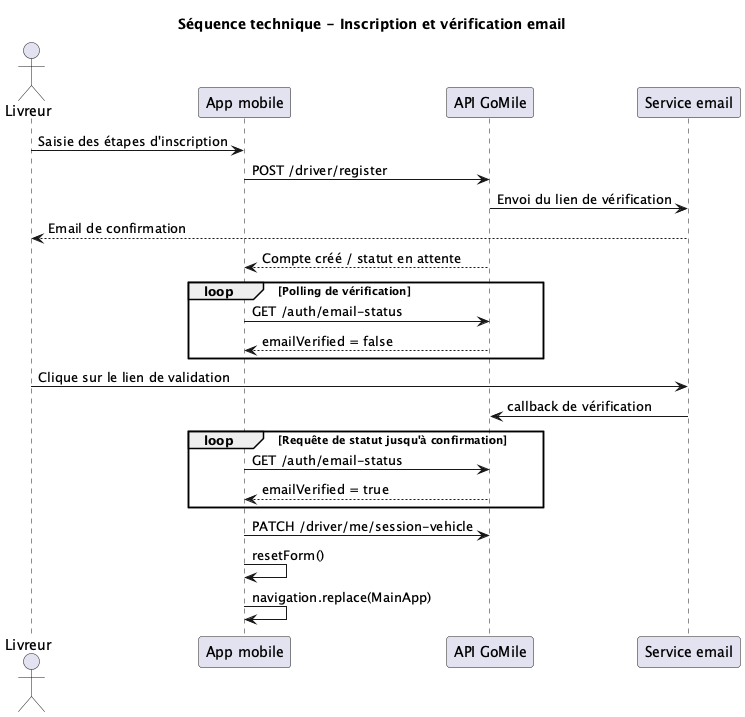
\includegraphics[width=0.95\textwidth]{../assets/app-mobile-registration-sequence.png}
    \caption{Séquence technique d'inscription avec vérification email}
\end{figure}

\subsection{Connexion et vérification email}

Après lancement de l'application, l'utilisateur arrive sur \texttt{LoginScreen}. Il saisit son identifiant (email ou téléphone) et son mot de passe.

\begin{itemize}
    \item Si le compte est valide, l'application ouvre directement l'espace principal.
    \item Si l'email n'est pas vérifié, l'utilisateur est redirigé vers \texttt{EmailVerificationScreen}.
\end{itemize}

Cet écran de vérification interroge périodiquement le backend. Une fois le mail confirmé via le lien reçu, l'application met à jour la session et redirige automatiquement vers le tableau de bord.

\begin{figure}[h!]
    \centering
    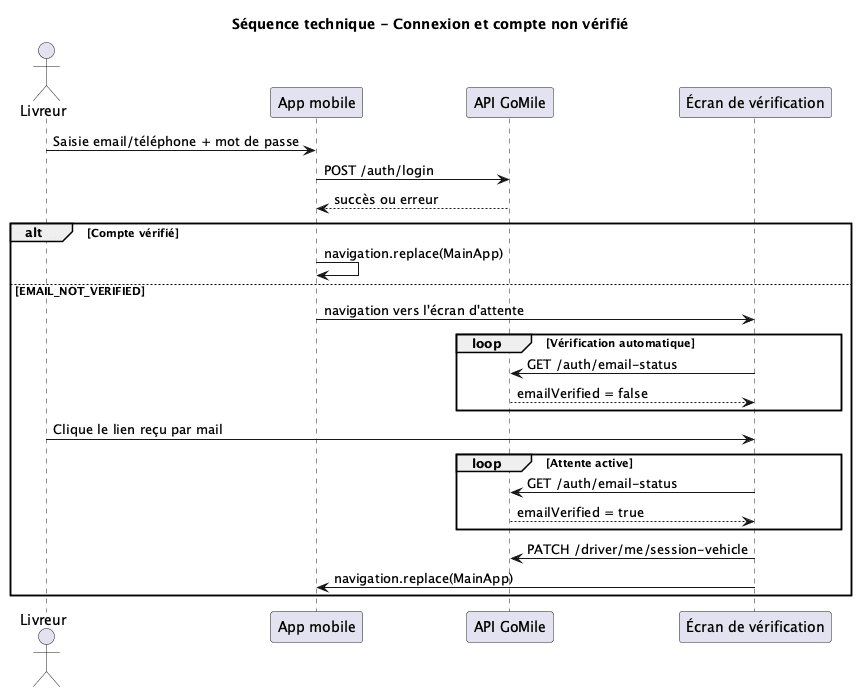
\includegraphics[width=0.95\textwidth]{../assets/app-mobile-login-sequence.png}
    \caption{Séquence technique de connexion avec gestion de l'email non vérifié}
\end{figure}

\subsection{Réinitialisation du mot de passe}

Depuis \texttt{LoginScreen}, l'action \texttt{Mot de passe oublié} ouvre le flux de réinitialisation:
\begin{itemize}
    \item envoi d'une demande de reset,
    \item réception d'un email,
    \item définition d'un nouveau mot de passe,
    \item retour à la connexion.
\end{itemize}

Cette séparation permet de garder un écran de connexion simple tout en offrant un parcours de récupération complet.

\begin{figure}[h!]
    \centering
    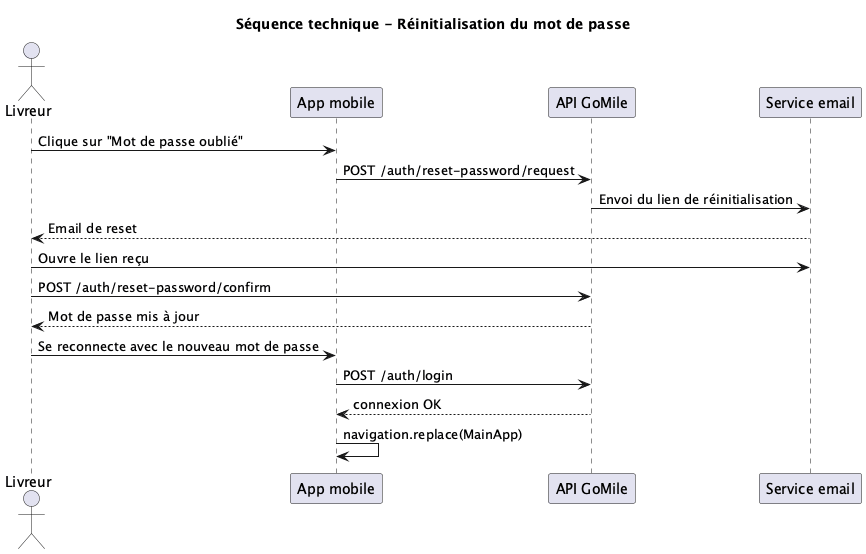
\includegraphics[width=0.95\textwidth]{../assets/app-mobile-reset-password-sequence.png}
    \caption{Séquence technique de réinitialisation du mot de passe}
\end{figure}

\subsection{Diagramme d'état global authentification}

Le diagramme d'état ci-dessous résume les transitions entre les états principaux: connexion, inscription, attente de vérification email, accès au dashboard, et retour après déconnexion ou reset du mot de passe.

\begin{figure}[h!]
    \centering
    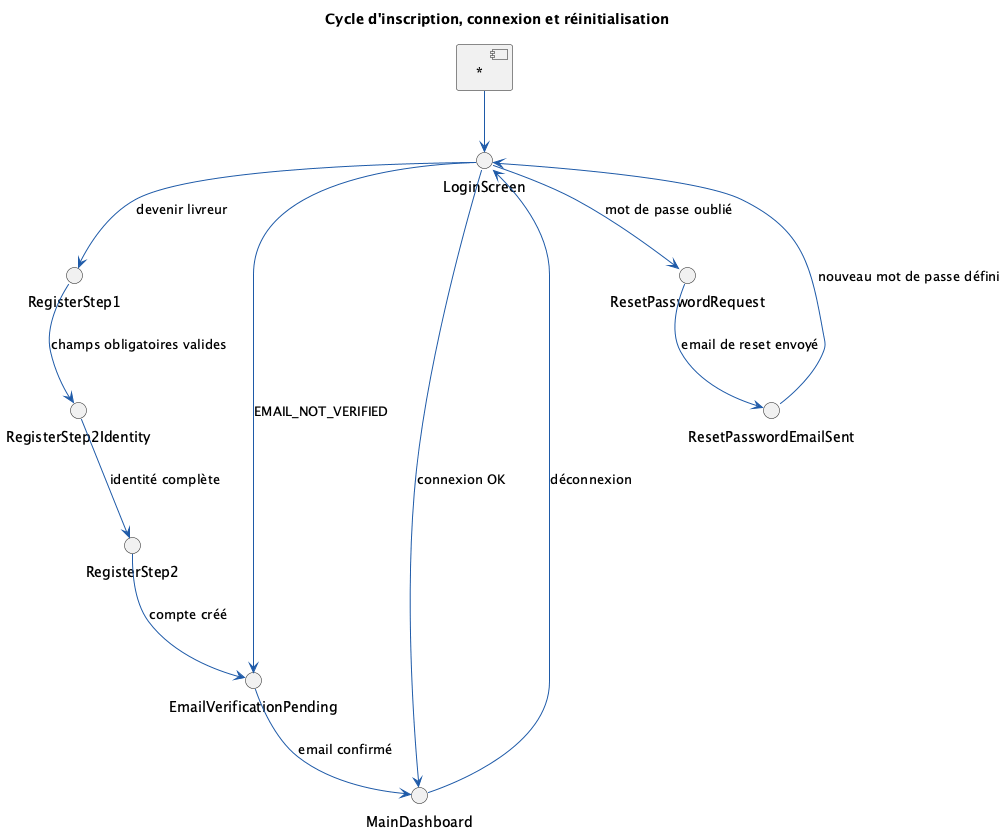
\includegraphics[width=0.95\textwidth]{../assets/app-mobile-auth-state.png}
    \caption{Diagramme d'état global du cycle inscription-connexion-reset}
\end{figure}

\subsection{Décisions UX abandonnées ou déplacées}

Les évolutions du parcours ont conduit à déplacer plusieurs éléments hors du tunnel d'inscription principal:
\begin{itemize}
    \item Les documents KYC ne sont plus demandés pendant les trois étapes d'inscription: ils sont traités après création du compte, depuis le profil.
    \item L'ancien écran de finalisation (ancien \texttt{RegisterStep4}) reste présent dans le code, mais n'est plus intégré au flux UX principal.
    \item La vérification SMS complète n'est pas activée à ce stade; une vérification de validité du numéro est appliquée, avec arbitrage coût/complexité sur les services externes.
\end{itemize}

\newpage
\subsection{Navigation et écrans post-connexion}

\subsubsection{Architecture de navigation principale (MainTabs)}

Une fois connecté, le livreur arrive sur \texttt{MainTabs.js}, qui constitue le cœur de l'application post-authentification. Cette structure repose sur:

\begin{description}
    \item[React Navigation Bottom Tab Navigator] organisation de quatre onglets principaux accessibles en permanence au bas de l'écran.
    \item[Stack Navigator implicite] chaque onglet peut avoir ses propres écrans enfants (ex: MissionDetailsScreen accessible depuis MissionsScreen).
    \item[Push Notifications] configuration des notifications à ce niveau, avec enregistrement du token et liaison WebSocket.
    \item[Suivi GPS] mise à jour de la position du livreur à intervalle régulier pour enrichir les suggestions de missions.
    \item[WebSocket (socket.io)] connexion établie ici pour recevoir les événements en temps réel (nouvelles missions, changements de statut).
\end{description}

\subsubsection{Header personnalisé avec toggle en ligne/hors ligne}

Le header \texttt{Header.js} affiche:
\begin{itemize}
    \item Le titre de la page courante (ex: <<TABLEAU DE BORD>>, <<MISSIONS>>).
    \item Un indicateur \texttt{EN LIGNE} / \texttt{HORS LIGNE} avec switch.
    \item Lorsque le livreur bascule \textbf{en ligne}, il devient visible dans les requêtes de mission; \textbf{hors ligne}, aucune mission ne lui est proposée.
    \item La transition repose sur un appel à \texttt{toggleDriverAvailability()} (endpoint PATCH \texttt{/driver/me/availability}).
    \item Sécurité: un livreur ne peut pas se mettre hors ligne s'il a une mission active en cours.
\end{itemize}

\textbf{Magasin partagé:} \texttt{useAvailabilityStore} (simple toggle Zustand) maintient l'état \texttt{isOnline} en mémoire de session.

\subsubsection{Écran 1: Tableau de Bord (Dashboard / TableauDeBord.js)}

\subsubsection{Purpose et composition}

Le Tableau de Bord est l'écran d'accueil principal post-connexion. Il présente:

\begin{itemize}
    \item \textbf{Carte interactive Google Maps} affichant:
    \begin{itemize}
        \item La position actuelle du livreur (marqueur bleu).
        \item Les missions disponibles à proximité (marqueurs rouges).
        \item Un cercle de rayon 1 km autour de la position courante.
    \end{itemize}
    \item \textbf{Widget de statistiques rapides}:
    \begin{itemize}
        \item Gains du jour (format: \texttt{XX.XX€}).
        \item Nombre de courses effectuées aujourd'hui.
    \end{itemize}
    \item \textbf{Overlay de missions proposées}: défilement horizontal des cartes mission les plus proches, avec bouton <<Voir détails>>.
\end{itemize}

\subsubsection{Logique de localisation et mise à jour}

À l'ouverture du Dashboard:
\begin{enumerate}
    \item Demande de permission de géolocalisation (\texttt{Location.requestForegroundPermissionsAsync}).
    \item Récupère la position courante avec précision \texttt{Balanced}.
    \item Appelle immédiatement \texttt{updateDriverLocation(lat, lng)} pour synchroniser la position backend (nécessaire pour la requête géospatiale ST\_DWithin).
    \item Charge le dashboard via \texttt{getDriverDashboard()} pour les statistiques du jour.
    \item Lance le hook de polling \texttt{useMissionsPoller({ fetchAll: false })} qui va rafraîchir les missions disponibles au focus et à intervalle régulier.
\end{enumerate}

\subsubsection{Intégration des stores et hooks}

\textbf{Stores utilisés:}
\begin{itemize}
    \item \texttt{useAvailabilityStore}: lecture de \texttt{isOnline} pour afficher/masquer les missions.
    \item \texttt{useMissionStore}: lecture de \texttt{availableMissions} pour afficher les marqueurs et les cartes.
\end{itemize}

\textbf{Hooks:}
\begin{itemize}
    \item \texttt{useMissionsPoller({ fetchAll: false })}: fetch unique des missions disponibles au premier focus de l'écran et au passage en ligne.
\end{itemize}

\textbf{Endpoints API appelés:}
\begin{itemize}
    \item \texttt{getDriverDashboard()}: GET \texttt{/driver/me/dashboard} → retourne \texttt{\{isOnline, todayEarnings, todayTrips\}}.
    \item \texttt{updateDriverLocation(lat, lng)}: PATCH \texttt{/driver/me/location} → envoie la position actuelle.
    \item \texttt{getAvailableMissions()}: GET \texttt{/driver/me/missions/available} → retourne tableau de missions.
\end{itemize}

\subsubsection{Interaction utilisateur}

\begin{itemize}
    \item \textbf{Tap sur une carte mission}: ouvre \texttt{MissionDetailsScreen} avec les détails complets.
    \item \textbf{Tap sur le bouton GPS}: recentre la carte sur la position courante.
    \item \textbf{Affichage hors ligne}: les missions ne sont pas visibles; message: <<Les missions proposées sont masquées hors ligne>>.
\end{itemize}

\subsection{Écran enfant: Détails Mission (MissionDetailsScreen)}

\subsubsection{Purpose et composition}

Cet écran affiche les détails complets d'une mission sélectionnée depuis le Tableau de Bord ou depuis l'écran Missions. L'utilisateur peut y accepter ou refuser la mission.

Contenu affiché:
\begin{itemize}
    \item Carte avec trajet pick-up → destination (Polyline).
    \item Nom du commerce, adresse pick-up, zone de livraison.
    \item Rémunération, distance estimée, durée.
    \item Boutons: REFUSER et ACCEPTER.
\end{itemize}

\subsubsection{Logique d'acceptation et refus}

\textbf{Accepter:}
\begin{enumerate}
    \item Appel API \texttt{acceptMission(missionId)}: POST \texttt{/driver/me/missions/\{id\}/accept}.
    \item Dispatch action Zustand \texttt{acceptMission(missionCard)} qui ajoute la mission à \texttt{missionQueue}.
    \item Navigation vers \texttt{MissionFocusScreen} pour débuter le suivi GPS en direct.
\end{enumerate}

\textbf{Refuser:}
\begin{enumerate}
    \item Alerte de confirmation: <<Cette mission sera retirée de ta liste>>.
    \item Dispatch action Zustand \texttt{declineMission(missionId)} qui:
    \begin{itemize}
        \item Ajoute l'ID à \texttt{declinedMissionIds}.
        \item Filtre la mission hors de \texttt{availableMissions}.
    \end{itemize}
    \item Navigation arrière.
\end{enumerate}

\subsubsection{Calcul du trajet et géocodage}

À l'ouverture:
\begin{itemize}
    \item Récupère la position courante du livreur.
    \item Appelle \texttt{getDrivingRoute([currentPos, pickupPos, dropoffPos])} pour obtenir la route optimale.
    \item Affiche distance formatée et durée estimée.
\end{itemize}

\textbf{Endpoints API:}
\begin{itemize}
    \item \texttt{acceptMissionApi(missionId)}: POST acceptation.
    \item \texttt{getDrivingRoute()}: calcul route (utilise service Google Maps ou routeur local).
\end{itemize}

\newpage
\subsection{Diagramme de flux: Navigation Tableau de Bord → Détails Mission → Focus}

\begin{figure}[H]
    \centering
    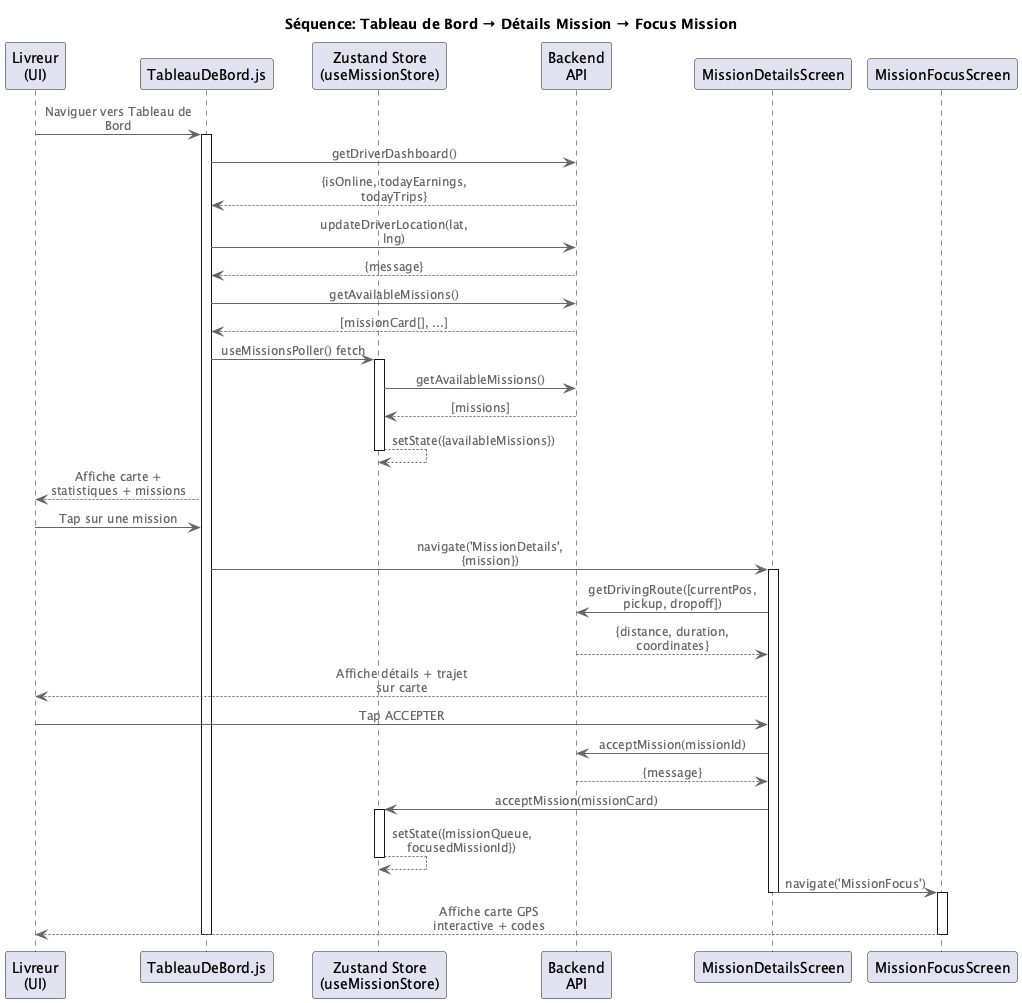
\includegraphics[width=0.9\textwidth]{../assets/app-mobile-dashboard-sequence.png}
    \caption{
        Séquence technique: le livreur arrive sur le Tableau de Bord, consulte une mission via MissionDetailsScreen, puis l'accepte pour passer en MissionFocusScreen et débuter le suivi GPS. Les stores Zustand maintiennent l'état entre chaque transition.
    }
    \label{fig:app-mobile-dashboard-sequence}
\end{figure}

\subsection{Diagramme d'état: Cycle de vie d'une mission acceptée}

\begin{figure}[H]
    \centering
    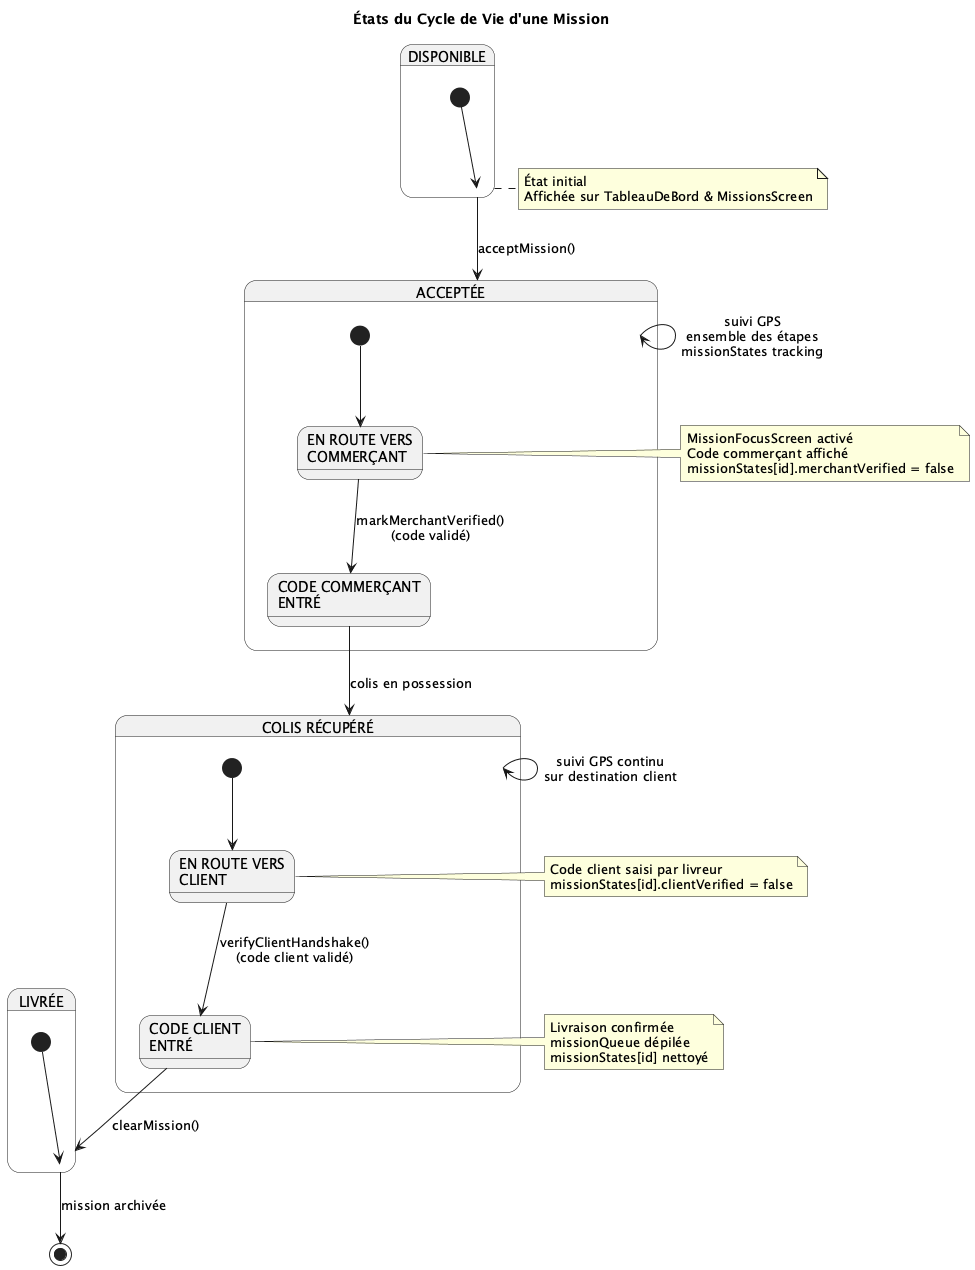
\includegraphics[width=0.9\textwidth]{../assets/app-mobile-mission-lifecycle.png}
    \caption{
        États d'une mission: disponible → acceptée (EN ROUTE vers commerçant) → récupérée (RÉCUPÉRÉ colis, EN ROUTE vers client) → livrée (LIVRÉ). Les codes marchant et client actent le passage entre états.
    }
    \label{fig:app-mobile-mission-lifecycle}
\end{figure}

\newpage
\subsection{Écran 2: Missions (MissionsScreen)}

\subsubsection{Purpose et organisation par onglets}

Cet écran centralise la gestion des missions sous trois onglets logiques:

\begin{description}
    \item[\textbf{Notifications Missions}] résumé du nombre de missions disponibles + horodatage du dernier rafraîchissement.
    \item[\textbf{Onglet 1: Missions en cours}] toutes les missions acceptées (état \texttt{active} dans \texttt{missionQueue}), avec bouton <<REPRENDRE LA MISSION>> redirigeant vers MissionFocusScreen.
    \item[\textbf{Onglet 2: Missions à proximité}] liste complète des missions disponibles avec bouton <<VOIR LES DÉTAILS>> ouvrant MissionDetailsScreen pour consultation avant acceptation.
    \item[\textbf{Onglet 3: Historique}] historique des livraisons (archivées) avec magasins et rémunérations.
\end{description}

Comportement selon le statut en ligne:
\begin{itemize}
    \item \textbf{En ligne}: affichage des trois onglets + banneau informatif.
    \item \textbf{Hors ligne}: banneau unique expliquant que les missions ne sont pas disponibles.
\end{itemize}

\subsubsection{Stores et intégration Zustand}

\textbf{Store \texttt{useMissionStore} - lectures:}
\begin{itemize}
    \item \texttt{availableMissions}: missions proposées à proximité (GET \texttt{/driver/me/missions/available}).
    \item \texttt{activeMissions}: missions en cours acceptées (GET \texttt{/driver/me/missions/active}).
    \item \texttt{historyMissions}: missions archivées (GET \texttt{/driver/me/missions/history}).
    \item \texttt{lastRefreshAt}: timestamp du dernier fetch.
    \item \texttt{isLoadingMissions}: indicateur de chargement.
\end{itemize}

\textbf{Store \texttt{useMissionStore} - actions:}
\begin{itemize}
    \item \texttt{acceptMission(mission)}: ajoute à \texttt{missionQueue} et définit comme focalisée.
    \item \texttt{declineMission(missionId)}: ajoute à \texttt{declinedMissionIds}, filtre hors de \texttt{availableMissions}.
    \item \texttt{fetchAvailableMissions()}: appel backend pour missions disponibles.
    \item \texttt{fetchAllMissions()}: appel bundle pour tous les états (disponibles + actives + historique).
\end{itemize}

\subsubsection{Polling et refresh}

Le hook \texttt{useMissionsPoller({ fetchAll: true })} gère:
\begin{itemize}
    \item Fetch unique au premier focus de MissionsScreen.
    \item Fetch au passage du livreur en ligne.
    \item Bouton <<RAFRAÎCHIR>> manuel appelant \texttt{refresh()}.
\end{itemize}

\textbf{Nouveau système (remplace le polling périodique):}
\begin{itemize}
    \item Les nouvelles missions arrivent via WebSocket (événement \texttt{order:new}) reçu dans MainTabs.
    \item Le hook ne sert plus au polling périodique, mais au chargement initial et refresh manuel.
    \item Gain: réduction de la charge réseau, mises à jour en temps réel via événements.
\end{itemize}

\subsubsection{Navigation et actions utilisateur}

\begin{itemize}
    \item \textbf{Tap <<VOIR LES DÉTAILS>>}: ouvre MissionDetailsScreen pour consultation et décision.
    \item \textbf{Tap <<REPRENDRE LA MISSION>>}: appelle \texttt{acceptMission()}, navigue immédiatement vers MissionFocusScreen.
    \item \textbf{Tap <<RAFRAÎCHIR>>}: appelle \texttt{refresh()} du hook de polling.
\end{itemize}

\subsection{Écran enfant: Focus Mission (MissionFocusScreen)}

\subsubsection{Purpose: suivi GPS en direct et vérification codes}

Cet écran est le cœur de la livraison. Il affiche:
\begin{itemize}
    \item \textbf{Carte interactive} avec:
    \begin{itemize}
        \item Marqueur bleu: position actuelle du livreur (mise à jour en temps réel).
        \item Marqueurs rouges: toutes les missions en cours (pick-up en rouge, livraison en rose).
        \item Polyline: trajet calculé vers la cible courante.
    \end{itemize}
    \item \textbf{Panneau bas} (collapsible) contenant:
    \begin{itemize}
        \item Sélecteur de mission (si plusieurs en cours).
        \item Code commerçant (affiché, non saisi).
        \item Bouton de validation commerçant.
        \item Champ saisie code client (après validation commerçant).
        \item Bouton de validation client.
    \end{itemize}
\end{itemize}

\subsubsection{Logique de vérification: deux étapes}

\textbf{Étape 1: Vérification commerçant}
\begin{enumerate}
    \item Livreur arrive au point de pick-up.
    \item Code commerçant est affiché via \texttt{getMissionPickupCode(missionId)}.
    \item Commerçant valide le code via son interface (pas de saisie livreur ici).
    \item Livreur tape le bouton <<VALIDER IDENTIFICATION COMMERÇANT>>.
    \item Action \texttt{markMerchantVerified(missionId)} active l'étape suivante.
    \item État: \texttt{missionStates[id].merchantVerified = true}.
\end{enumerate}

\textbf{Étape 2: Vérification client}
\begin{enumerate}
    \item Livreur arrive au point de livraison.
    \item Champ de saisie code client devient actif (6 chiffres).
    \item Client fournit le code (via SMS ou interface app).
    \item Livreur saisit le code.
    \item Appel API \texttt{verifyClientHandshake(missionId, code)}: POST \texttt{/driver/me/missions/\{id\}/handshake/client/verify}.
    \item Si succès: action \texttt{markClientVerified(missionId)}.
    \item Alerte: <<Mission terminée, Livraison confirmée!>>.
    \item Action \texttt{clearMission(missionId)}: dépile de \texttt{missionQueue}, met à jour \texttt{focusedMissionId}.
\end{enumerate}

\subsubsection{Suivi GPS continu}

À l'ouverture du MissionFocusScreen:
\begin{enumerate}
    \item Demande permission géolocalisation.
    \item Lance \texttt{watchPositionAsync()}: mise à jour position toutes les 5 secondes (distance minimale: 10 m).
    \item À chaque nouvelle position:
    \begin{itemize}
        \item Met à jour \texttt{currentPosition} (état local).
        \item Recalcule la route vers la cible courante via \texttt{getDrivingRoute()}.
        \item Affiche distance et durée estimée.
    \end{itemize}
    \item Arrêt au démontage du composant.
\end{enumerate}

\subsubsection{Sélecteur de missions (si plusieurs en file)}

Si \texttt{missionQueue.length > 1}:
\begin{itemize}
    \item Affiche composant \texttt{MissionPicker} permettant de basculer entre missions.
    \item À chaque sélection, \texttt{setFocusedMission(id)} met à jour \texttt{focusedMissionId}.
    \item La carte et le panneau se réajustent instantanément.
    \item Affichage du statut de chaque mission: EN ROUTE, RÉCUPÉRÉ, LIVRÉ.
\end{itemize}

\subsubsection{Endpoints API utilisés}

\begin{itemize}
    \item \texttt{getMissionPickupCode(missionId)}: GET \texttt{/driver/me/missions/\{id\}/handshake/pickup-code} → code commerçant.
    \item \texttt{verifyClientHandshake(missionId, code)}: POST \texttt{/driver/me/missions/\{id\}/handshake/client/verify} → validation livraison.
    \item \texttt{getDrivingRoute([coords])}: calcul route.
\end{itemize}

\newpage
\subsection{Diagramme de flux: Acceptation mission → Focus → Vérification codes}

\begin{figure}[H]
    \centering
    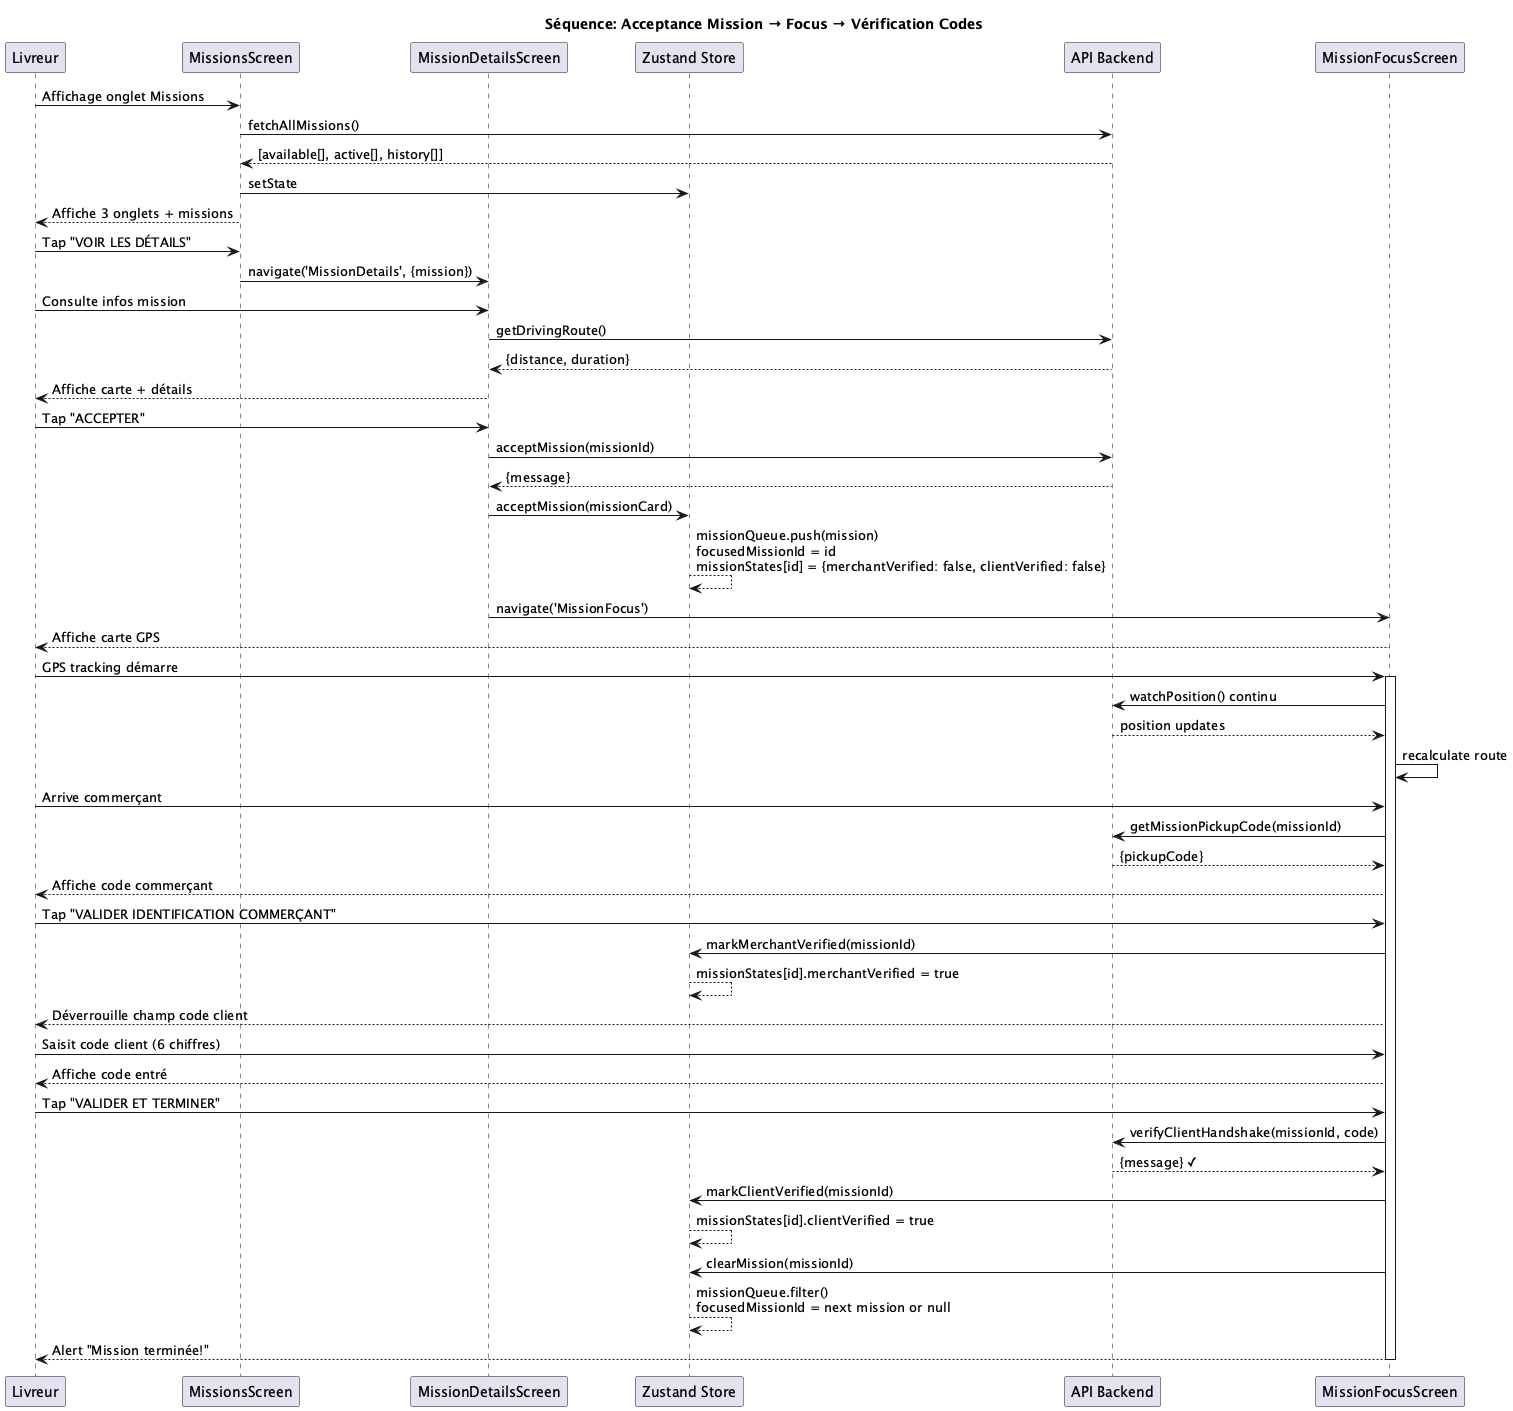
\includegraphics[width=0.95\textwidth]{../assets/app-mobile-missions-acceptance-sequence.png}
    \caption{
        Séquence technique: depuis MissionsScreen, le livreur accepte une mission via MissionDetailsScreen. La mission s'ajoute à la file (missionQueue). MissionFocusScreen s'affiche avec suivi GPS. Codes commerçant et client sont vérifiés séquentiellement, puis la mission est archivée.
    }
    \label{fig:app-mobile-missions-acceptance-sequence}
\end{figure}

\subsection{Diagramme d'état: Transition états mission dans MissionFocusScreen}

\begin{figure}[H]
    \centering
    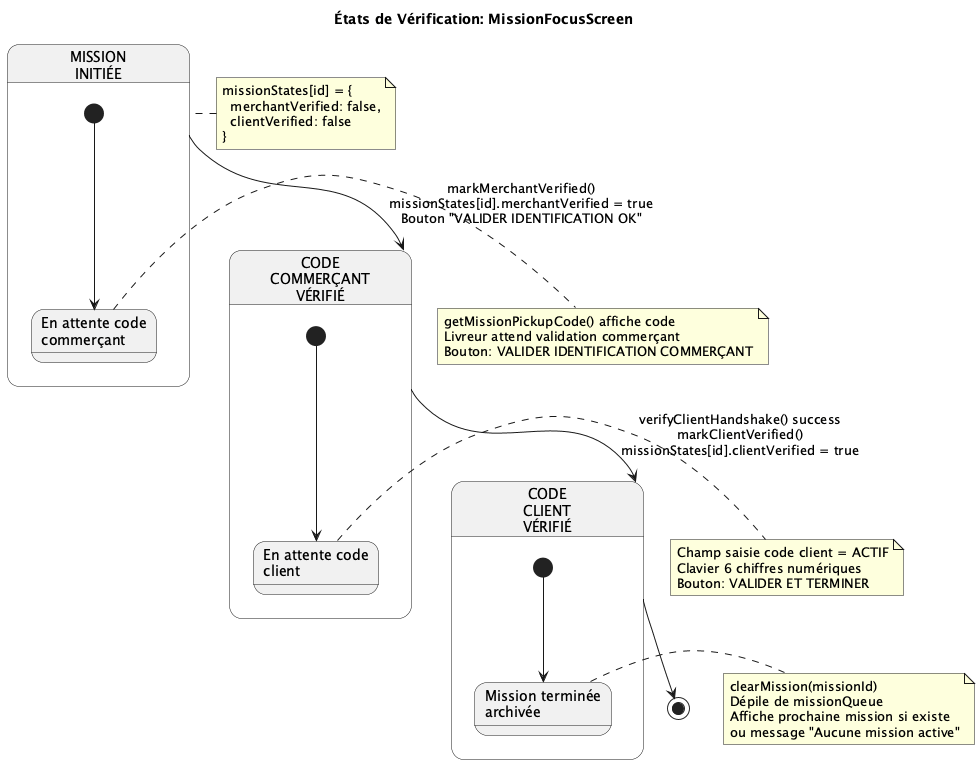
\includegraphics[width=0.9\textwidth]{../assets/app-mobile-mission-verification-states.png}
    \caption{
        États de vérification dans MissionFocusScreen: INITIÉE → COMMERÇANT VÉRIFIÉ (merchantVerified=true) → CLIENT VÉRIFIÉ (clientVerified=true) → TERMINÉE. À chaque étape, le panneau se met à jour pour afficher le code suivant ou le message de fin.
    }
    \label{fig:app-mobile-mission-verification-states}
\end{figure}

\newpage
\subsection{Écran 3: Portefeuille (WalletScreen)}

\subsubsection{Purpose: gestion du solde et retrait}

Le Portefeuille affiche les gains du livreur et permet les demandes de virement. Composants:

\begin{itemize}
    \item \textbf{Carte solde principal}: affiche le solde disponible et le montant en attente de paiement.
    \item \textbf{Historique des transactions}: liste des crédits et débits avec dates, montants, statuts.
    \item \textbf{Bouton <<Demander un virement>>}: ouvre modal de retrait.
    \item \textbf{Modal de retrait}: saisie montant, boutons rapides (25%, 50%, 75%, 100%), validation.
\end{itemize}

\subsubsection{Modal de retrait}

À l'ouverture du modal:
\begin{enumerate}
    \item Affiche solde disponible.
    \item Champ saisie montant (\texttt{TextInput}, clavier décimal).
    \item Boutons rapides calculant pourcentages du solde:
    \begin{itemize}
        \item 25\%, 50\%, 75\%, 100\% pré-calculs.
        \item Champ se remplit automatiquement.
    \end{itemize}
    \item Validation et vérification:
    \begin{itemize}
        \item Montant doit être > 0.
        \item Montant doit être $\leq$ solde disponible.
    \end{itemize}
    \item Appel API \texttt{requestWithdrawal(amount)}: POST \texttt{/driver/me/wallet/withdrawals}.
    \item Sur succès: alerte confirmation + rechargement du solde.
\end{enumerate}

\subsubsection{Endpoints API}

\begin{itemize}
    \item \texttt{getWallet()}: GET \texttt{/driver/me/wallet} → \texttt{\{balance, pendingAmount, currency\}}.
    \item \texttt{getWalletEntries()}: GET \texttt{/driver/me/wallet/entries} → historique transactions.
    \item \texttt{requestWithdrawal(amount)}: POST \texttt{/driver/me/wallet/withdrawals} → demande virement.
\end{itemize}

\subsection{Écran 4: Profil (ProfileScreen)}

\subsubsection{Purpose: gestion identité et KYC}

Le Profil réunit les informations personnelles du livreur et l'accès au parcours KYC. Composants:

\begin{itemize}
    \item \textbf{Carte identité principale}:
    \begin{itemize}
        \item Avatar circulaire (stocké sur S3 ou placeholder).
        \item Nom et prénom.
        \item Note moyenne (rating) et nombre total de courses.
        \item Véhicule actuel (BIKE, SCOOTER, etc.).
        \item Numéro de code GoMile unique.
        \item Statut en ligne (ONLINE / OFFLINE).
    \end{itemize}
    \item \textbf{Sélecteur de véhicule}: change le type de véhicule actif pour la session via \texttt{updateSessionVehicle(vehicleType)}.
    \item \textbf{Widget KYC}: affiche le statut de vérification (NOT\_SUBMITTED, PENDING, APPROVED, REJECTED) avec badge coloré et CTA vers KYCScreen.
    \item \textbf{Section parrainage}: affiche code de parrainage et bouton pour partager avec amis.
    \item \textbf{Bouton déconnexion}: termine la session, clear tokens, retour écran LoginScreen.
\end{itemize}

\subsubsection{Statut KYC sur ProfileScreen}

Chaque état affiche une configuration visuelle distincte:

\begin{itemize}
    \item \textbf{NOT\_SUBMITTED}: badge orange, icône alerte, message <<Ajoute tes documents>>, CTA <<Compléter mon KYC>>.
    \item \textbf{PENDING}: badge bleu, icône horloge, message <<En cours de vérification>>, CTA <<Voir mes documents>>.
    \item \textbf{APPROVED}: badge vert, icône checkmark, message <<Compte vérifié>>, CTA <<Voir les détails>>.
    \item \textbf{REJECTED}: badge rouge, icône X, message <<Documents refusés>>, CTA <<Corriger mes documents>>.
\end{itemize}

Tap sur le widget: redirection vers KYCScreen avec le statut courant.

\subsubsection{Endpoints API}

\begin{itemize}
    \item \texttt{getDriverProfile()}: GET \texttt{/driver/me/profile} → infos perso.
    \item \texttt{updateSessionVehicle(vehicleType)}: PATCH \texttt{/driver/me/session-vehicle}.
    \item \texttt{getMyKycStatus()}: GET \texttt{/driver/me/kyc} → statut KYC.
    \item \texttt{getMyReferral()}: GET \texttt{/driver/me/referral} → code parrainage.
    \item \texttt{logout()}: clear tokens (local storage).
\end{itemize}

\newpage
\subsection{Diagramme de flux: Wallet (solde → retrait → confirmation)}

\begin{figure}[H]
    \centering
    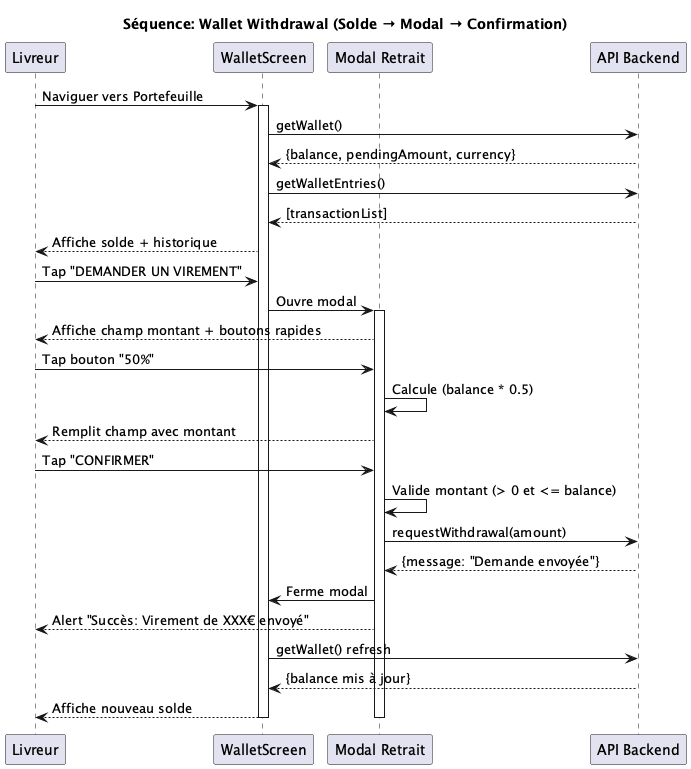
\includegraphics[width=0.9\textwidth]{../assets/app-mobile-wallet-withdrawal-sequence.png}
    \caption{
        Séquence: livreur consulte solde, ouvre modal retrait, calcule montant (rapide ou saisie), valide. API confirme, solde est mis à jour.
    }
    \label{fig:app-mobile-wallet-withdrawal-sequence}
\end{figure}

\subsection{Diagramme d'état: Profil et transitions KYC}

\begin{figure}[H]
    \centering
    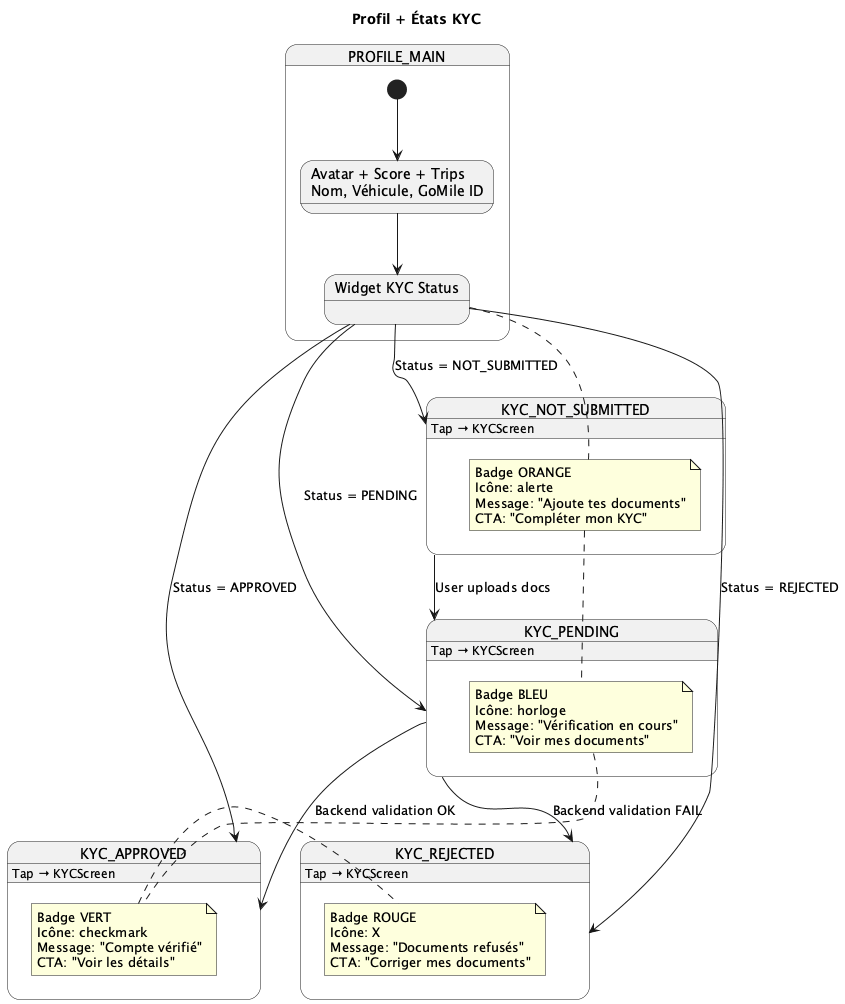
\includegraphics[width=0.85\textwidth]{../assets/app-mobile-profile-kyc-states.png}
    \caption{
        État du profil: affichage des infos de base. Widget KYC avec 4 états colorés (NOT\_SUBMITTED → PENDING → APPROVED ou REJECTED). Tap sur widget navigue vers KYCScreen.
    }
    \label{fig:app-mobile-profile-kyc-states}
\end{figure}

\newpage
\section{Écran enfant: KYC (KYCScreen)}

KYCScreen est l'écran dédié à la vérification d'identité et à la gestion des documents. C'est ici que le livreur téléverse les pièces justificatives requises.

\subsection{Slots et types de documents}

GoMile demande 5 emplacements (slots) de documents:

\begin{description}
    \item[\textbf{IDENTITY}] accepte <<\textbf{Carte nationale d'identité}>> (CNI) OU <<\textbf{Passeport}>>. Un seul des deux suffit.
    \item[\textbf{DRIVING\_LICENSE}] permis de conduire.
    \item[\textbf{REGISTRATION\_CARD}] carte grise (immatriculation véhicule).
    \item[\textbf{RIB}] relevé bancaire (IBAN/RIB pour virements).
    \item[\textbf{JUSTIFICATIF\_DOMICILE}] justificatif de domicile de moins de 3 mois.
\end{description}

L'utilisateur peut téléverser des fichiers images (PNG, JPEG) ou PDF.

\subsection{États de vérification d'un document}

Chaque document dans un slot a quatre états possibles:

\begin{description}
    \item[\textbf{Non fourni}] aucun fichier uploadé; puce grise; CTA <<Ajouter document>>.
    \item[\textbf{En attente d'examen}] document uploadé mais pas encore vérifiée par backend; icône horloge bleu; puce bleu.
    \item[\textbf{Vérifié}] backend a validé le document; icône checkmark vert; puce vert; badge <<Vérifié~\checkmark>>.
    \item[\textbf{Refusé}] backend a rejeté le document; icône X rouge; puce rouge; badge <<Refusé — à corriger>> + raison de rejet.
\end{description}

\subsection{Statut KYC global}

Le statut global du compte KYC a aussi quatre états:

\begin{description}
    \item[\textbf{NOT\_SUBMITTED}] aucun document n'a été soumis; affichage: badge <<KYC à compléter>>, sous-titre <<Téléverse tes documents>>, icône alerte.
    \item[\textbf{PENDING}] au moins un document soumis, en attente de vérification backend; badge <<Vérification en cours>>, sous-titre <<Examen sous 48h>>, icône horloge.
    \item[\textbf{ACCEPTED}] tous les documents requis ont été validés; badge <<Compte vérifié>>, sous-titre <<Tu as accès à tous les missions>>, icône checkmark vert.
    \item[\textbf{REJECTED}] un ou plusieurs documents refusés; badge <<Documents refusés>>, sous-titre <<Corrige-les et resoumets>>, icône X rouge.
\end{description}

\subsection{Workflow d'upload de document}

\subsubsection{Étape 1: Sélection du fichier}

\begin{enumerate}
    \item Livreur tap sur slot vide ou sur document existant pour modifier.
    \item Modal: choix <<Caméra>>, <<Galerie photo>>, ou <<Fichier>>.
    \item Livreur sélectionne source et choisit/prend le fichier.
    \item Module \texttt{media-picker}: applique permissions, retourne URI du fichier.
\end{enumerate}

\subsubsection{Étape 2: Presignage URL S3}

\begin{enumerate}
    \item Appel API \texttt{presignDocument(filename, contentType)}: POST \texttt{/driver/me/documents/presign}.
    \item Backend retourne: \texttt{\{uploadUrl, fileUrl\}}.
    \item \texttt{uploadUrl} est une URL S3 signée (temporaire, ~5 min).
    \item \texttt{fileUrl} est l'URL finale du fichier stocké.
\end{enumerate}

\subsubsection{Étape 3: Upload S3 direct}

\begin{enumerate}
    \item Utilise \texttt{uploadFileToPresignedUrl(uploadUrl, file, contentType)}.
    \item Envoie fichier directement vers S3 via l'URL signée (bypass backend, plus rapide).
    \item Indicateur loading: <<Envoi en cours...>>.
    \item Sur succès: puce de l'état passe à <<En attente d'examen>> (bleu).
\end{enumerate}

\subsubsection{Étape 4: Liaison document au slot}

\begin{enumerate}
    \item Appel API \texttt{createMyDocument(type, fileUrl)}: POST \texttt{/driver/me/documents}.
    \item Backend enregistre le document lié au slot.
    \item État du document: \texttt{\{id, type, url, verified: false, rejectionReason: null, createdAt\}}.
\end{enumerate}

\subsubsection{Étape 5: Soumission KYC (optionnel)}

\begin{enumerate}
    \item Livreur voit tous les documents uploadés.
    \item Bouton <<SOUMETTRE MA DEMANDE KYC>>: appel API \texttt{submitMyKyc()}: POST \texttt{/driver/me/kyc}.
    \item Statut passe à PENDING; backend commence vérification.
\end{enumerate}

\subsection{Suppression document}

Livreur peut supprimer un document via bouton \texttt{deleteDocument(documentId)}: DELETE \texttt{/driver/me/documents/\{id\}}.

La puce revient à <<Non fourni>>.

\subsection{Endpoints API pour KYC}

\begin{itemize}
    \item \texttt{getMyKycStatus()}: GET \texttt{/driver/me/kyc} → \texttt{\{status: 'NOT\_SUBMITTED'|'PENDING'|'ACCEPTED'|'REJECTED', latestSubmission\}}.
    \item \texttt{getMyDocuments()}: GET \texttt{/driver/me/documents} → liste des documents uploadés.
    \item \texttt{presignDocument(filename, contentType)}: POST \texttt{/driver/me/documents/presign} → \texttt{\{uploadUrl, fileUrl\}}.
    \item \texttt{uploadFileToPresignedUrl(uploadUrl, file, contentType)}: PUT vers S3 (hors API GoMile).
    \item \texttt{createMyDocument(type, fileUrl)}: POST \texttt{/driver/me/documents} → enregistre document.
    \item \texttt{deleteDocument(documentId)}: DELETE \texttt{/driver/me/documents/\{id\}}.
    \item \texttt{submitMyKyc()}: POST \texttt{/driver/me/kyc} → soumet au backend pour vérification.
\end{itemize}

\newpage
\subsection{Diagramme de flux: Upload document KYC complet}

\begin{figure}[H]
    \centering
    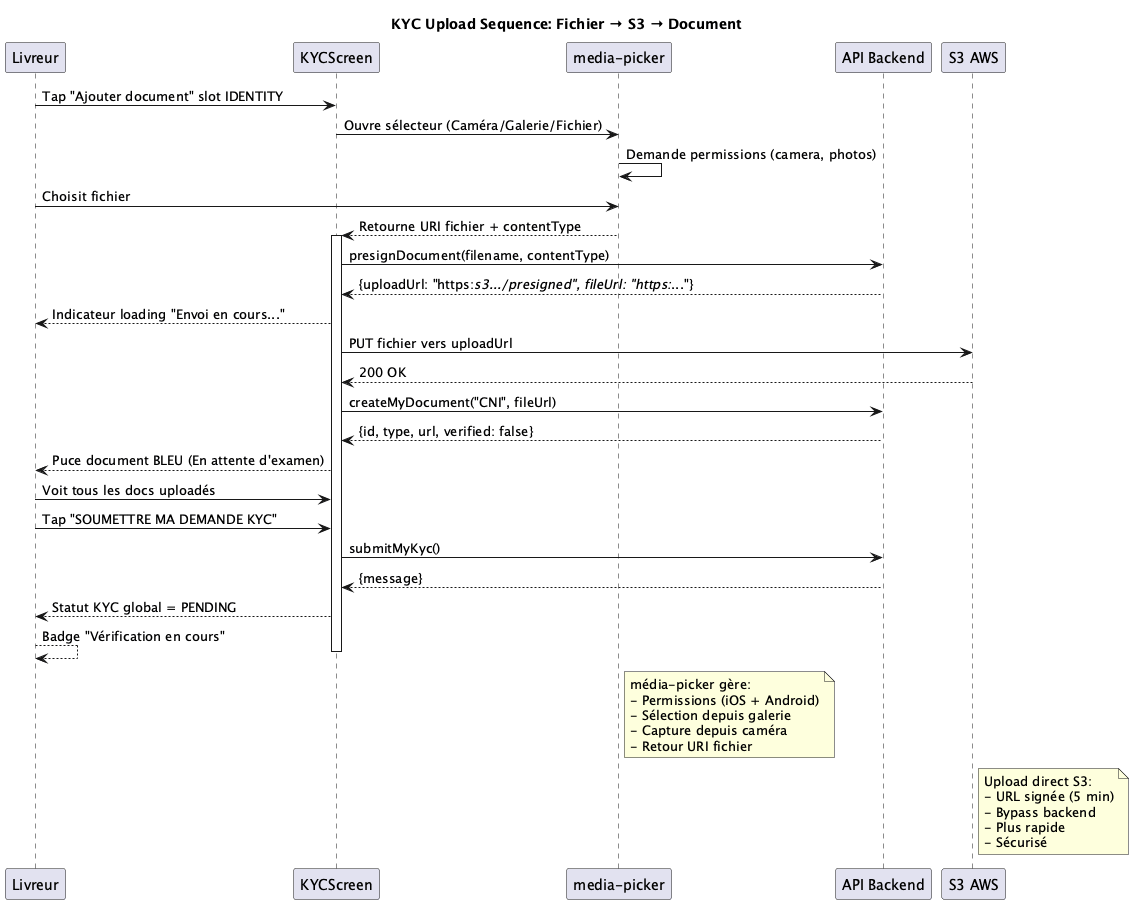
\includegraphics[width=0.95\textwidth]{../assets/app-mobile-kyc-upload-sequence.png}
    \caption{
        Séquence technique: livreur sélectionne fichier → presignage URL S3 → upload direct S3 → création document backend. État passe à <<En attente d'examen>>. Soumission optionnelle vérrouille les modifications.
    }
    \label{fig:app-mobile-kyc-upload-sequence}
\end{figure}

\subsection{Diagramme d'état: KYC global + transitions documents}

\begin{figure}[H]
    \centering
    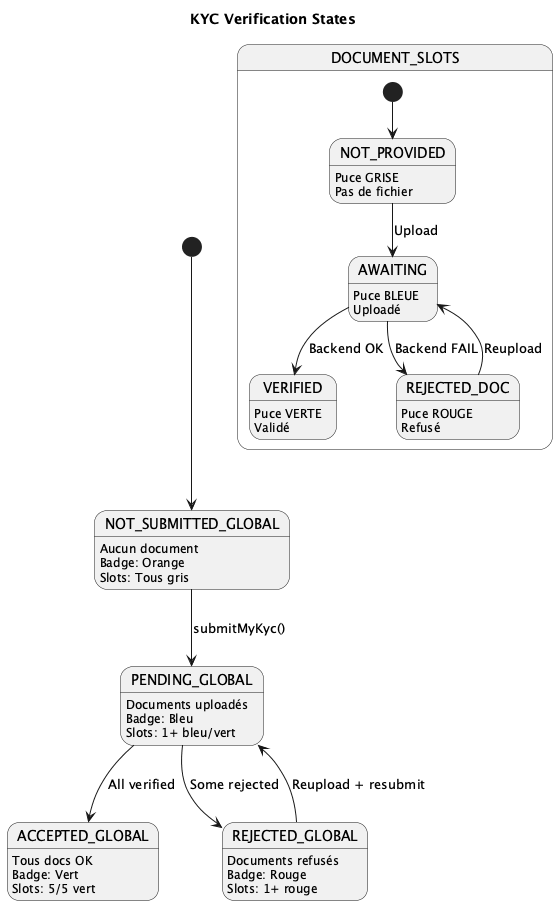
\includegraphics[width=0.9\textwidth]{../assets/app-mobile-kyc-verification-states.png}
    \caption{
        États: NOT\_SUBMITTED → PENDING (documents uploadés) → ACCEPTED (tous vérifiés) ou REJECTED (révision nécessaire). Chaque slot a ses propres états (Non fourni, En attente, Vérifié, Refusé). Livreur peut reupload et resubmit.
    }
    \label{fig:app-mobile-kyc-verification-states}
\end{figure}

\newpage
\section{Services et stores partagés}

\subsection{useMissionStore (Zustand)}

Le store central pour la gestion des missions:

\begin{description}
    \item[\textbf{missionQueue}] tableau des missions acceptées en cours de livraison.
    \item[\textbf{focusedMissionId}] ID de la mission actuellement suivie (MissionFocusScreen).
    \item[\textbf{missionStates}] objet: \texttt{\{[missionId]: \{merchantVerified, clientVerified\}\}}.
    \item[\textbf{availableMissions}] missions proposées à proximité.
    \item[\textbf{activeMissions}] missions acceptées (alias de missionQueue pour l'affichage).
    \item[\textbf{historyMissions}] missions archivées/livrées.
    \item[\textbf{lastRefreshAt}] timestamp dernier fetch.
    \item[\textbf{isLoadingMissions}] indicateur chargement.
\end{description}

Actions principales:
\begin{itemize}
    \item \texttt{acceptMission(mission)}: ajoute à missionQueue, définit focusée.
    \item \texttt{declineMission(missionId)}: ajoute à declinedMissionIds.
    \item \texttt{markMerchantVerified(id)}: marque commerçant vérifié.
    \item \texttt{markClientVerified(id)}: marque client vérifié.
    \item \texttt{clearMission(id)}: dépile mission, met à jour focusedMissionId.
    \item \texttt{setFocusedMission(id)}: bascule mission focalisée.
    \item \texttt{fetchAvailableMissions()}: GET API missions disponibles.
    \item \texttt{fetchAllMissions()}: GET API tous les états (disponibles + actives + historique).
    \item \texttt{initStore()}: restaure missions actives au démarrage.
\end{itemize}

\subsection{useAvailabilityStore (Zustand)}

Store simple pour le statut en ligne/hors ligne:

\begin{itemize}
    \item \texttt{isOnline}: booléen état courant.
    \item \texttt{setOnlineStatus(boolean)}: action mise à jour.
    \item \texttt{toggleOnlineStatus()}: toggle action.
\end{itemize}

Intégration: tout écran lit \texttt{isOnline} pour afficher/masquer les éléments mission-dépendants.

\subsection{useMissionsPoller (Hook personnalisé)}

Hook gérant le fetch des missions avec filtrage par écran:

\begin{itemize}
    \item Paramètre \texttt{\{ fetchAll: boolean \}}.
    \item \texttt{fetchAll = false}: dashboard uniquement missions disponibles (rapide).
    \item \texttt{fetchAll = true}: MissionsScreen charge tous les états.
    \item Fetch unique au premier focus de l'écran OU passage en ligne.
    \item Bouton refresh manuel via retour action \texttt{\{ refresh() \}}.
    \item Les nouvelles missions arrivent aussi via WebSocket (events \texttt{order:new} dans MainTabs).
\end{itemize}

\subsection{socketService (WebSocket)}

Connexion socket.io au backend pour événements temps réel:

\begin{description}
    \item[\textbf{connectSocket(token)}] établit connexion; emmet \texttt{join-driver} avec driverId.
    \item[\textbf{Events reçus}]
    \begin{itemize}
        \item \texttt{order:new}: nouvelle mission disponible → fetch + notification push locale.
        \item \texttt{driver:status}: changement statut driver côté serveur (ex: forcer offline).
    \end{itemize}
    \item[\textbf{disconnectSocket()}] ferme connexion (logout ou app termination).
\end{description}

Socket reste actif pendant toute la durée de session (MainTabs et enfants).

\subsection{driver-client.ts (API endpoints)}

Tous les appels API sont centralisés ici. Endpoints post-connexion:

\begin{itemize}
    \item \texttt{getDriverDashboard()}: GET \texttt{/driver/me/dashboard}.
    \item \texttt{toggleDriverAvailability()}: PATCH \texttt{/driver/me/availability}.
    \item \texttt{updateDriverLocation(lat, lng)}: PATCH \texttt{/driver/me/location}.
    \item \texttt{getAvailableMissions()}: GET \texttt{/driver/me/missions/available}.
    \item \texttt{acceptMission(id)}: POST \texttt{/driver/me/missions/\{id\}/accept}.
    \item \texttt{getActiveMissions()}: GET \texttt{/driver/me/missions/active}.
    \item \texttt{getMissionHistory()}: GET \texttt{/driver/me/missions/history}.
    \item \texttt{getMissionPickupCode(id)}: GET \texttt{/driver/me/missions/\{id\}/handshake/pickup-code}.
    \item \texttt{verifyClientHandshake(id, code)}: POST \texttt{/driver/me/missions/\{id\}/handshake/client/verify}.
    \item \texttt{getWallet()}: GET \texttt{/driver/me/wallet}.
    \item \texttt{getWalletEntries()}: GET \texttt{/driver/me/wallet/entries}.
    \item \texttt{requestWithdrawal(amount)}: POST \texttt{/driver/me/wallet/withdrawals}.
    \item \texttt{getDriverProfile()}: GET \texttt{/driver/me/profile}.
    \item \texttt{updateSessionVehicle(vehicleType)}: PATCH \texttt{/driver/me/session-vehicle}.
    \item \texttt{getMyKycStatus()}: GET \texttt{/driver/me/kyc}.
    \item \texttt{getMyDocuments()}: GET \texttt{/driver/me/documents}.
    \item \texttt{presignDocument(filename, contentType)}: POST \texttt{/driver/me/documents/presign}.
    \item \texttt{createMyDocument(type, fileUrl)}: POST \texttt{/driver/me/documents}.
    \item \texttt{deleteDocument(id)}: DELETE \texttt{/driver/me/documents/\{id\}}.
    \item \texttt{submitMyKyc()}: POST \texttt{/driver/me/kyc}.
\end{itemize}

Gestion d'erreurs centralisée: redirection si token invalide, parsing des erreurs backend, retry logic.

\subsection{Récapitulatif: flux complet d'une session livreur}

\begin{enumerate}
    \item Connexion: LoginScreen → EmailVerificationScreen → MainTabs.
    \item MainTabs initialise: notifications push, WebSocket, position GPS, fetch missions initiales.
    \item Livreur navigue entre onglets (TableauDeBord, Missions, Portefeuille, Profil).
    \item Accepte une mission → MissionDetailsScreen → MissionFocusScreen.
    \item Suivi GPS en direct, codes vérifiés séquentiellement.
    \item Mission livrée → archivée, gains crédités au portefeuille.
    \item Livreur consulte portefeuille, peut demander retrait.
    \item Livreur manage profil, KYC, données personnelles.
    \item Déconnexion: suppression tokens, fermeture WebSocket.
\end{enumerate}
